\chapter{Experimentación}

\section{Materiales}

En la presente sección enunciamos los diversos recursos que hemos utilizado y ayudarán a entender cómo se llevaron a cabo los experimentos tanto previos en el laboratorio como los del presente trabajo.

\subsection{Corpus de entrenamiento}

Para poder entrenar no solo los modelos de lenguaje generados por la AWD-LSTM, 
sino también generar los embeddings dentro del modelo de Word2Vec se utilizó un 
corpus grande de texto en español. En particular, se decidió utilizar el corpus 
llamado \textit{all\_wikis}, proveniente del repositorio de textos en español 
\textit{large\_spanish\_corpus}, creado por Jose Cañete\footnote{https://huggingface.co/datasets/josecannete/large\_spanish\_corpus}.
Este corpus está compuesto por fragmentos extraídos de distintas wikis en español, 
como \textit{Wikipedia}, \textit{Wikinews}, \textit{Wikiquotes} y muchas más, completando un corpus de $28.109.484$ filas, 
correspondiente a una oración por cada una. A menos que se indique lo contrario, 
los modelos serán entrenados con este corpus.

Además, todos los gráficos relacionados a la metrica \textit{perplexity} fueron realizados sobre el \textit{dataset} de validación del corpus, dejando asi el \textit{dataset} de entrenamiento exclusivamente para el entrenamiento de los modelos. Para más informacion sobre como se dividió el corpus, ver la sección \ref{sec:validacion_base}.


\subsection{Experimentos de similitud}

Como mencionamos anteriormente, el eje principal de este trabajo es el de analizar el 
comportamiento de modelos generados a partir de la arquitectura AWD-LSTM luego de incorporarles 
información cognitiva. Para esto, se decidió comparar los embeddings obtenidos de los modelos 
resultantes con dos bases de datos que nos permiten obtener información sobre juicios de similitud 
humanos entre pares de palabras, SWOW-RP y Multi-Simlex. A continuación, se muestra como fueron 
preprocesados estos repositorios y de qué manera luego fueron comparados con los embeddings 
generados tanto en el presente trabajo como los de trabajos previos en el laboratorio.

\subsubsection{Multi-Simlex}

Como habíamos denotado previamente, Multi-Simlex es un repositorio que cuenta con respuestas 
sobre juicios de similitud entre pares de palabras brindados por 10 anotadores distintos. 
Estos sujetos dieron para cada par de palabras un valor de similitud entre $0$ y $6$, donde $0$ 
se considera muy poca similitud y $6$ extremadamente similares. Para poder tener una métrica 
más compacta con la cual comparar los \textit{embeddings}, se decidió tomar el promedio de los valores 
dados por estos anotadores como nuestra medida de similitud final.

Luego, para realizar la comparación con los \textit{embeddings} de los modelos, se calcula la correlación 
de \textit{Spearman} de todos los pares de palabras del repositorio, comparando, por un lado, el promedio 
de los valores dados por estos anotadores y, por el otro, la similitud coseno entre los 
\textit{embeddings} de ambas palabras, extraídos a partir del modelo.

\subsubsection{SWOW-RP}

Por otro lado, SWOW-RP es una base de datos resultante de varias tareas de asociación de palabras, 
donde a partir de una palabra inicial (\textit{cue}), los sujetos contestaban con las primeras tres 
palabras que se les venían a la mente.

A partir de ahí, el repositorio brinda información ya procesada sobre estas tareas, ya sea 
para únicamente la primera respuesta o para las tres. Por ejemplo, brinda la frecuencia de 
una respuesta sobre una \textit{cue} o incluso la probabilidad condicional de haber elegido una 
respuesta a partir de una \textit{cue} en particular. En nuestro caso, se tomó la decisión de tomar 
esta última como medida de similitud entre dos pares de palabras, ya que tomar la frecuencia 
hubiera sido imposible, al tener cantidades distintas de respuestas para cada \textit{cue}. Además se 
eligió contar con la versión de los datos que tiene en cuenta las tres respuestas para mayor 
abarcabilidad.

Luego, para tener una idea más en profundidad del efecto que la información cognitiva puede 
generar sobre los \textit{embeddings}, en este caso se optó por dividir los pares de palabras de este 
repositorio en dos. Por un lado, se agruparon los pares de palabras en donde ambas palabras 
estuvieran presentes en los cuentos; es decir, las palabras que recibieron atributos cognitivos 
durante el reentrenamiento. En el caso de que algunas de las palabras del par no incluyera 
información cognitiva, sería agrupada en el grupo restante.

Por último, se calculó la correlación de \textit{Spearman} de la misma manera que en el caso anterior, 
con la salvedad de que, con el objetivo de obtener mayor rigurosidad estadística, se decidió 
hacer esta comparación no sobre el espacio de pares de palabras total, sino sobre un muestreo 
de $1000$ pares generados con reposición unas $100$ veces.

\section{Trabajos previos}

\label{sec:trabajos_previos}

Previo a este trabajo, dentro del laboratorio de la mano del licenciado Fermin Travi se estuvo 
investigando sobre la incidencia de la información cognitiva sobre otro tipo de modelos previos 
a la arquitectura AWD-LSTM, en este caso, Word2Vec.

Haciendo hincapié en el mismo, se utilizó una arquitectura de Word2Vec basada en \textit{skip-grams} y 
se entrenó al modelo utilizando como corpus base el mismo corpus aprovechado en este trabajo, 
valiéndose del 100\% del mismo durante el entrenamiento por una cantidad de 5 épocas.

Luego, los \textit{embeddings} resultantes del modelo fueron comparados con los repositorios de 
juicios de valor humanos presentados anteriormente, calculando la correlación entre los 
\textit{embeddings} y los datos de los repositorios, tal y como se observa en la figura siguiente:

\begin{figure}[H]
    \centering
    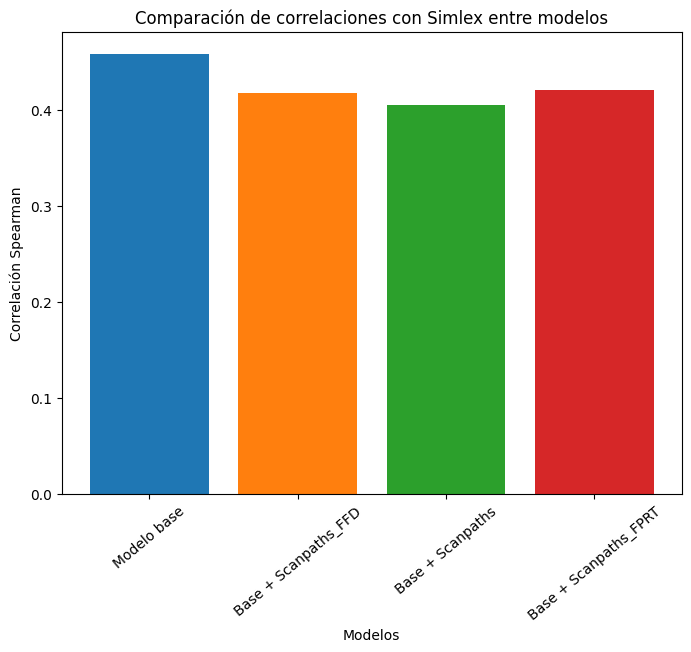
\includegraphics[width=0.8\textwidth]{imagenes/simlex_word2vec.png}
    \caption{Correlaciones entre distintos modelos de Word2Vec con los juicios de valor generados 
    por Multi-Simlex. Entre los modelos comparados se encuentran un modelo base implementado a 
    partir de \textit{skip-grams}, y 3 modelos reentrenados a partir de este, uno con los \textit{scanpaths} sin 
    ninguna métrica asociada y otros dos con los \textit{scanpaths} y las métricas FFD y FPRT asociadas 
    respectivamente.}
    \label{fig:simlex_word2vec}
\end{figure}

En particular, para el caso de Multi-Simlex, el modelo de Word2Vec generado a partir de \textit{skip-grams} 
reportó una correlación de \textit{Spearman} de $0,458$, la cual se utilizará en los experimentos venideros 
como base a la cual comparar los modelos generados por la AWD-LSTM. Además, se evidencia que 
la correlación empeora levemente al reentrenar el modelo con la información cognitiva, lo 
cual se considera esperable que ocurra al haber una gran cantidad de palabras que no se 
vieron influenciadas por el reentrenamiento. Sin embargo, se puede observar que este 
decaimiento es levemente menor en los modelos con las métricas presentes.

\subsection{Reentrenamiento}

Con este modelo base, a su vez, se decidió reentrenar el modelo de \textit{embeddings} 
añadiendo información generada a partir de movimientos oculares, haciendo uso 
de los \textit{scanpaths} generados por los experimentos de información cognitiva. Estos 
fueron reentrenados por una cantidad de 5 épocas valiéndose del 100\% de estos 
textos, introduciendo información sobre los movimientos oculares de los sujetos 
durante la lectura de los mismos.

Luego, los \textit{embeddings} generados por estos modelos fueron comparados con los datos 
del repositorio SWOW-RP, brindando los siguientes resultados:

\begin{figure}[H]
    \centering
    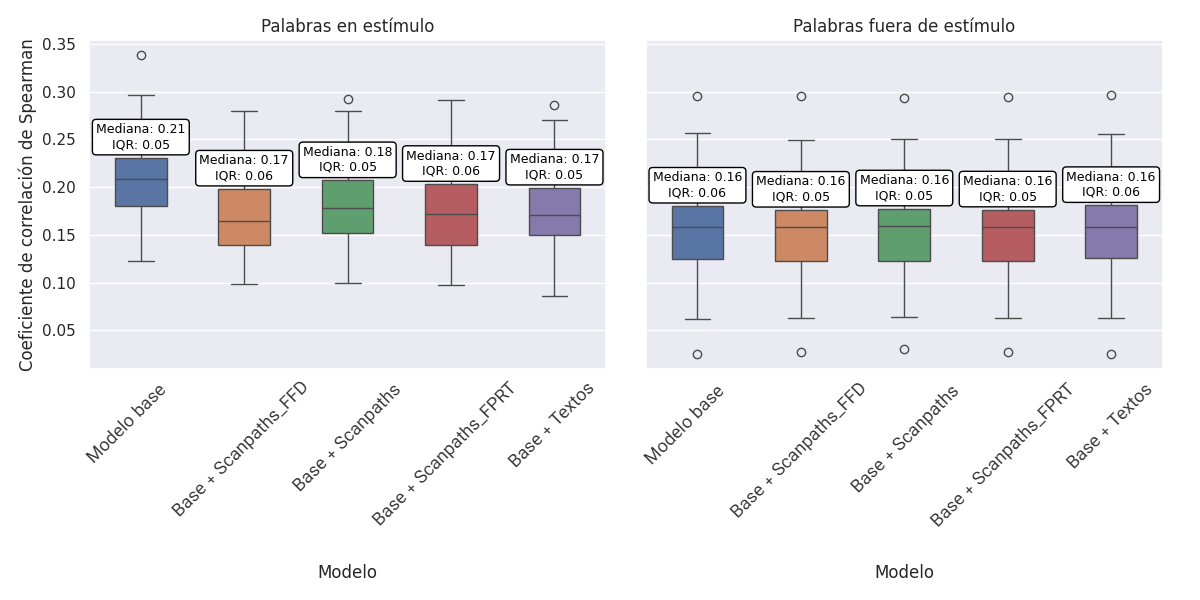
\includegraphics[width=1\textwidth]{imagenes/swow_word2vec.png}
    \caption{Correlaciones entre distintos modelos de Word2Vec y los juicios de similitud 
    generados a partir del repositorio SWOW-RP. La comparación parte con los mismos modelos 
    comparados con Multi-Simlex en la figura \ref{fig:simlex_word2vec}, sin embargo en este caso, se le añade el 
    modelo reentrenado con los textos originales de los cuentos.}
    \label{fig:swow_word2vec}
\end{figure}

Como se puede observar, los modelos reentrenados con los \textit{scanpaths} muestran una peor 
correlación con SWOW-RP comparados con el modelo original, indicando de cierta manera 
que con esta forma de comparación los \textit{embeddings} reentrenados parecen captar peor las 
similitudes entre los pares de palabras obtenidos en el repositorio. Esto al menos, para 
el caso de las palabras en estímulo, o sea las palabras dentro del vocabulario de los 
\textit{scanpaths}. Para el resto de palabras dentro del vocabulario del modelo, no parecen haber 
cambios sustanciales.

\section{Validación de implementación base}

\subsection{Comparación entre implementaciones de AWD-LSTM}

Tal y como se comentó en secciones anteriores, luego de obtener la implementación base 
de la arquitectura AWD-LSTM, se propuso validarla con otra implementación confiable que 
nos permita constatar que el código funciona correctamente. En este caso, se utilizó la 
implementación de la librería \textit{Fastai}.

Para realizar esta comparación, se decidió realizar un experimento entrenando dos 
modelos distintos: uno a partir de la herramienta brindada por \textit{Fastai} y otro 
entrenandolo a partir de la implementación base, con el objetivo de poder corroborar 
que ambos modelos sean parecidos en términos de \textit{performance} (validando empíricamente 
contra la implementación base). Durante el correr de las épocas de entrenamiento de ambos 
modelos, se tomó nota de la \textit{performance}, utilizando la \textit{perplexity} como métrica de los 
mismos frente al dataset de validación. Ambos modelos fueron entrenados utilizando 
uno de los corpus empleados en la experimentación del trabajo original de la AWD-LSTM 
\parencite{merity2017regularizingoptimizinglstmlanguage}, llamado \textit{Penn Treebank Dataset}, el cual engloba una serie de 
artículos en inglés del \textit{Wall Street Journal}, llegando a cubrir una 
cantidad de $38.219$ oraciones.

En particular, ambos modelos fueron entrenados durante $500$ épocas y se los configuró 
de manera tal que los modelos resultantes fueran los más parecidos posibles. Incluso se u
tilizó el mismo tokenizador, proveniente de la librería \textit{Fastai}, para que el vocabulario 
resultante fuera el mismo y los modelos pudieran ser comparables.

A pesar de esto, debido a las limitaciones de ambas implementaciones, hubo ciertas 
diferencias en la configuración:

\begin{itemize}
    \item Mientras que el \textit{learning rate} del modelo base se mantuvo en su valor por defecto 
    ($30$), en el caso del modelo de Fastai se decidió ejecutar con un \textit{learning rate} 
    de $5\text{e-}3$ (valor recomendado en el ejemplo de uso de la herramienta). Valores mucho más 
    altos, cercanos al \textit{learning rate} de la implementación base, no concluían en resultados 
    satisfactorios, ni siquiera comparables a los del trabajo original.
    \item Por otro lado, mientras que el modelo base se entrenó utilizando como optimizador 
    el algoritmo de NTASGD (ver \textcite{merity2017regularizingoptimizinglstmlanguage}), el modelo de 
    \textit{Fastai} se entrenó utilizando un optimizador ADAM, ya que la librería no presenta 
    dicho optimizador.
\end{itemize}

\subsubsection{Resultados}

\begin{figure}[H]
    \centering
    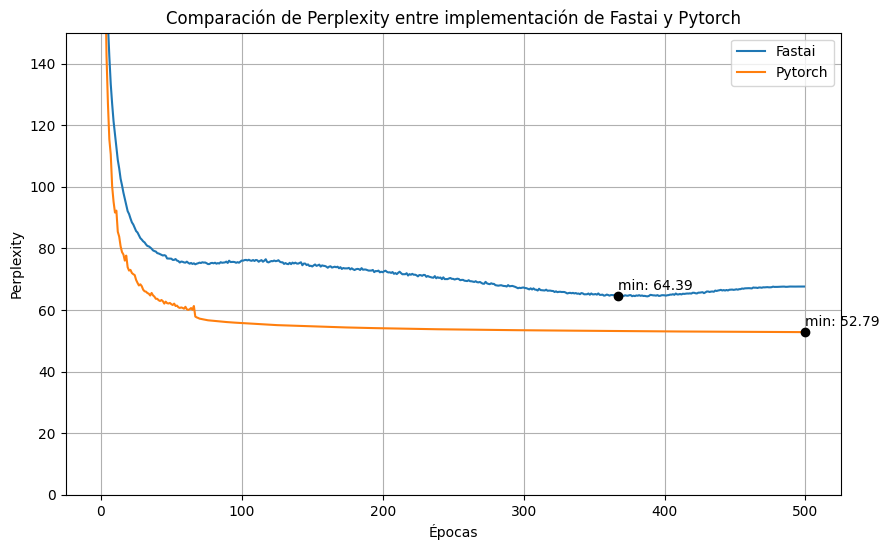
\includegraphics[width=0.8\textwidth]{imagenes/validacion_modelo.png}
    \caption{Comparación de la capacidad predictiva de dos modelos generados a partir 
    de una arquitectura AWD-LSTM a lo largo de las épocas. Uno de ellos fue generado 
    haciendo uso de la librería \textit{Fastai} mientras que el otro fue originado a partir 
    de nuestra implementación base en \textit{Pytorch}.}
    \label{fig:validacion_modelo}
\end{figure}

Como se puede observar en la figura \ref{fig:validacion_modelo}, con el correr de las épocas, no solo la 
\textit{performance} del modelo base generado en \textit{PyTorch} se asemeja al de su contraparte 
implementado con la librería \textit{Fastai}, sino que también se denota una mejora en la 
\textit{performance} frente a su contraparte a lo largo de las épocas.

\subsubsection{Síntesis}

A partir de esto, se concluyó que la implementación base de la AWD-LSTM genera resultados 
parecidos al de la implementación generada a partir de herramientas más consolidadas 
como las presentadas por la librería \textit{Fastai}, pudiendo constatar a esta implementación 
como un punto de partida válido para nuestras experimentaciones.

\section{Generación del modelo base}

\label{sec:modelo_base}

Ya contando con nuestra implementación de la AWD-LSTM adaptada a las necesidades de este 
trabajo, para poder cumplir con nuestro objetivo de analizar la performance de la 
arquitectura luego del reentrenamiento con datos provenientes de movimientos oculares 
fue necesario contar con un modelo base.

Para poder obtener el mismo, entrenamos la LSTM con el corpus \textit{all\_wikis} (rejunte de textos 
provenientes de \textit{Wiki-media}) presentado previamente.

\subsection{Comparación con Word2Vec}

Como primer acercamiento para hallar nuestro modelo base, se decidió generar un modelo 
utilizando toda la información brindada por el corpus, sin variar ningún otro hiperparámetro 
en particular. El entrenamiento del mismo se realizó durante 8 épocas y se extrajeron los 
\textit{embeddings} resultantes de la capa correspondiente en la red neuronal.

Luego, se comparó la similitud entre los \textit{embeddings} con la información de los juicios de 
Multi-Simlex al igual que en el caso de Word2Vec, en un principio con la hipótesis de 
poder observar una similitud mayor a los juicios humanos en comparación al modelo previo, 
ya que estamos hablando de una arquitectura posterior en el tiempo.

\subsubsection{Resultados}

\begin{figure}[H]
    \centering
    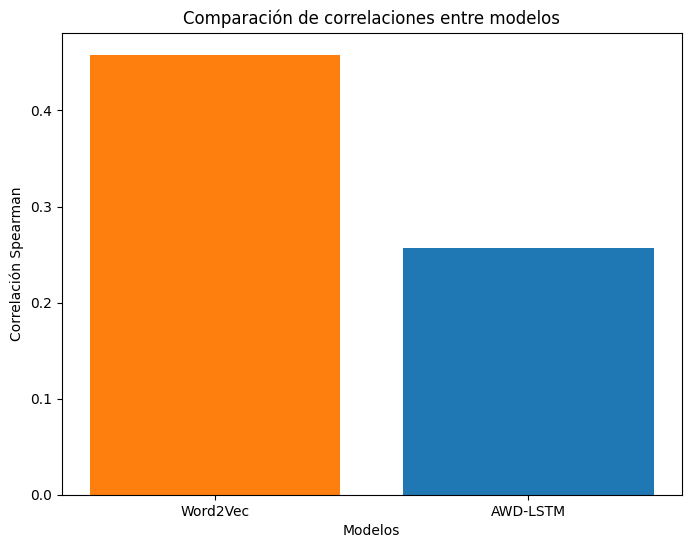
\includegraphics[width=0.72\textwidth]{imagenes/comparacion_w2v_lstm.png}
    \caption{Comparación de correlaciones con Multi-Simlex entre el modelo base 
    generado a partir de Word2Vec y un modelo construido sobre la arquitectura AWD-LSTM, 
    utilizando el 100\% del corpus de entrenamiento.}
    \label{fig:comparacion_w2v_lstm}
\end{figure}

Se puede evidenciar que, al contrario de lo que se suponía, el modelo generado a partir 
de la AWD-LSTM presenta una correlación peor ($0,257$) con los \textit{embeddings} humanos que su 
contraparte generada con Word2Vec ($0,458$), al menos para el caso de Multi-Simlex.

\subsubsection{Síntesis}

A partir de lo visto, este resultado evidencia (aún de manera no concluyente) que nuestra 
hipótesis inicial sobre la mejor capacidad de captar similitudes entre pares de palabras 
del modelo AWD-LSTM con respecto a Word2Vec podría ser errónea. Sin embargo, 
intuimos a su vez, que será necesario generar otros modelos de AWD-LSTM para tener 
resultados definitivos.

\subsection{Variando hiperparámetros}

En vista de los resultados del primer modelo, se tomó la decisión de variar los hiperparámetros 
ligeramente. El primero de ellos que nos interesó variar fue la cantidad de épocas con las 
cuales se entrena al mismo. Sin embargo, esto no nos pareció viable debido al gran tamaño 
del corpus utilizado, ya que esto implicaba un consumo de tiempo muy grande en el entrenamiento 
del modelo, de alrededor de $12$ horas cada época con un tamaño de batch de $30$. Por lo tanto, 
se optó por también reducir el porcentaje del corpus empleado, permitiendo así aumentar la 
cantidad de épocas.

En consecuencia, para el siguiente modelo se decidió permanecer con los mismos hiperparámetros, 
únicamente aumentando la cantidad de épocas de $8$ a $50$ y disminuyendo el porcentaje del corpus 
utilizado de 100\% a 10\%, con el objetivo de observar si la similitud con Multi-Simlex 
aumenta o se mantiene en un número comparable con el modelo anterior.

Adicionalmente, para este experimento calculamos la correlación con los \textit{embeddings} humanos 
al correr de las épocas, junto con la \textit{perplexity}, para ver de qué manera estas evolucionan 
a lo largo del tiempo.

\subsubsection{Resultados}

\begin{figure}[H]
    \centering
    \begin{subfigure}[b]{0.8\textwidth}
        \centering
        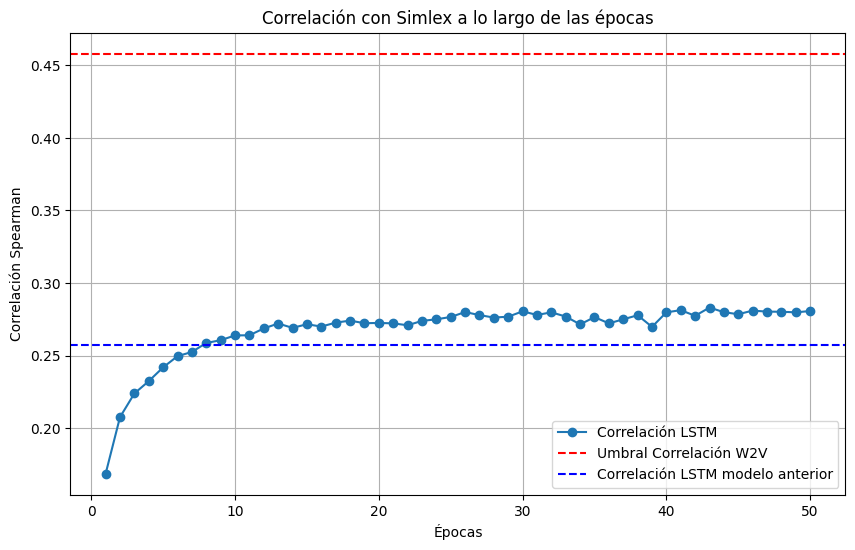
\includegraphics[width=1\textwidth]{imagenes/simlex_corr_10per.png}
        \caption{}
        \label{fig:simlex_corr_10per.png}
    \end{subfigure}
    \hfill
    \begin{subfigure}[b]{0.8\textwidth}
        \centering
        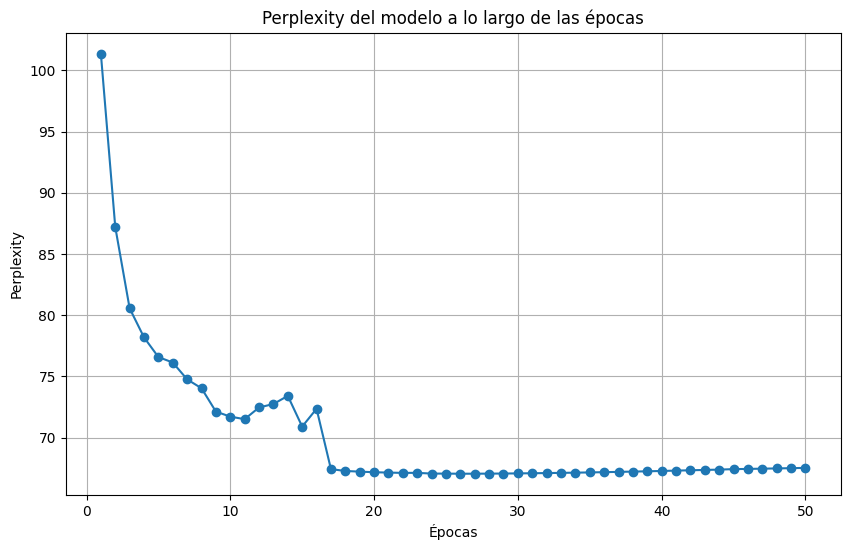
\includegraphics[width=1\textwidth]{imagenes/perp_10per.png}
        \caption{}
        \label{fig:perp_10per.png}
    \end{subfigure}
    \caption{En A, correlación con Multi-Simlex a lo largo de las épocas para el modelo con 
    una menor porcentaje de corpus de entrenamiento pero una mayor cantidad de épocas 
    entrenadas. Se grafica consigo la correlación de los modelos de la Figura \ref{fig:comparacion_w2v_lstm} para 
    facilitar la comparación. En B, se grafica la \textit{perplexity} del mismo modelo con el correr 
    de las épocas.}
    \label{fig:10per}
\end{figure}

Dentro del gráfico que mide correlación con Multi-Simlex (Figura \ref{fig:simlex_corr_10per.png}) podemos observar que, 
a pesar de que no se llega a pasar el umbral generado por los resultados con Word2Vec, la 
correlación a lo largo de las épocas termina superando ligeramente aquella del primer 
modelo AWD-LSTM presentado, finalizando el entrenamiento con una correlación de $0,281$.

Por otro lado, la \textit{perplexity} a lo largo de las épocas (Figura \ref{fig:perp_10per.png}) 
evidencia una reducción constante de la misma, mostrando que el modelo está mejorando su 
capacidad predictiva a lo largo de las épocas (al menos hasta la época $17$, donde el 
modelo parece estancarse).

\subsubsection{Síntesis}

Reducir el tamaño del corpus y aumentar la cantidad de épocas mejoró ligeramente la 
correlación entre los \textit{embeddings}, sin llegar aún al umbral estipulado por Word2Vec. 
Sin embargo, nos permite evidenciar que aumentar el tamaño del corpus no es 
proporcional a la correlación con los juicios de similitud humanos, por lo que 
se tomó la decisión de a partir de ahora seguir insistiendo con un tamaño de 
corpus del 10\% mientras se prueban otras opciones.

\subsection{Reduciendo el Learning Rate}

Para el siguiente modelo, valiéndose de los resultados anteriores, se eligió reducir el 
\textit{learning rate} que se aplica en el entrenamiento de $30$ a un número menor 
($3\text{e-3}$), con el objetivo de intentar mejorar el aprendizaje del modelo, 
potencialmente evitando el estancamiento de su \textit{perplexity}. En este caso, se decidió 
entrenar el modelo solamente con 25 épocas.

\subsubsection{Resultados}

\begin{figure}[H]
    \centering
    \begin{subfigure}[b]{0.8\textwidth}
        \centering
        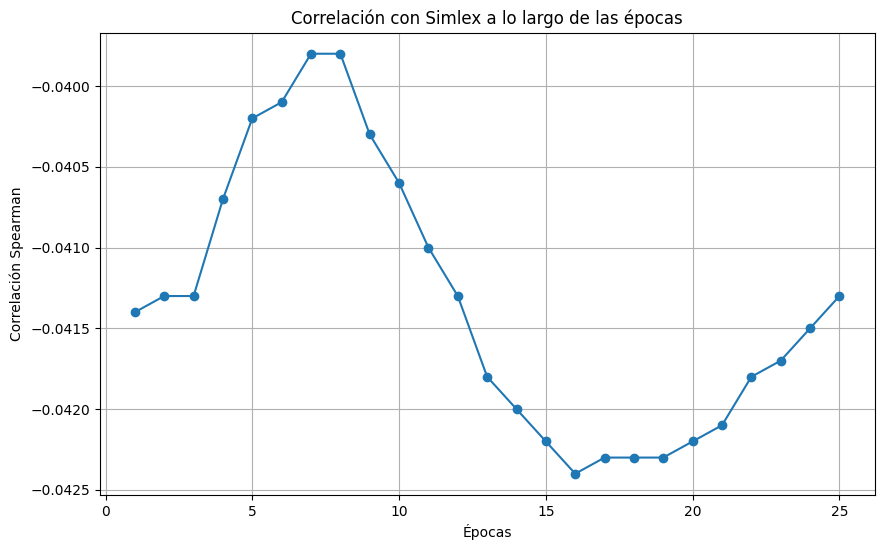
\includegraphics[width=1\textwidth]{imagenes/simlex_corr_lrreducido.png}
        \caption{}
        \label{fig:simlex_corr_lrreducido.png}
    \end{subfigure}
    \hfill
    \begin{subfigure}[b]{0.8\textwidth}
        \centering
        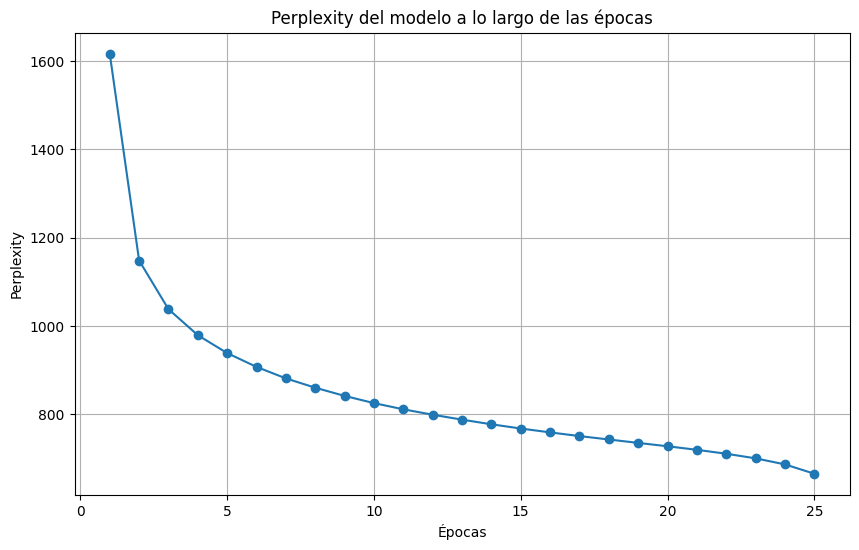
\includegraphics[width=1\textwidth]{imagenes/perp_lrreducido.png}
        \caption{}
        \label{fig:perp_lrreducido.png}
    \end{subfigure}
    \caption{En A, correlación del modelo entrenado con un \textit{learning rate} reducido con 
    Multi-Simlex. Por otro lado, en B se grafica la capacidad predictiva del modelo 
    durante el entrenamiento utilizando la \textit{perplexity} como métrica.}
    \label{fig:lrreducido}
\end{figure}

En lo que a \textit{perplexity} del modelo se refiere (Figura \ref{fig:perp_lrreducido.png}), se puede evidenciar que con un 
\textit{learning rate} menor el modelo no llega a estancarse. Sin embargo, con la cantidad de 
épocas dada no se llega a los niveles de \textit{perplexity} obtenidos en el modelo anterior, 
ya que se observa una mejora lenta de la misma.

Por otro lado, los resultados de la correlación con Multi-Simlex (Figura \ref{fig:simlex_corr_lrreducido.png}) no parecen 
mostrar resultados comparables a los anteriores modelos, posiblemente debido al poco 
aprendizaje realizado por el modelo durante el entrenamiento.

\subsubsection{Síntesis}

Luego de contemplar los últimos modelos, se puede notar que un \textit{learning rate} como el que 
se utiliza en la LSTM originalmente genera cierto estancamiento en la \textit{performance} del 
modelo, incluso utilizando el algoritmo inherente de la AWD-LSTM que varía el 
\textit{learning rate} de manera aleatoria con el pasar de las épocas. Por otro lado, si 
se reduce este hiperparámetro a un número más estándar dentro de la academia, el 
modelo no se llega a estancar, pero su \textit{performance} no es comparable a la de sus 
predecesores. Con esto en mente, se pensó en modificar la forma en la que varía 
el \textit{learning rate} con el fin de obtener lo mejor de los dos mundos.

\subsection{Modificación de la variación del Learning Rate}

A partir de lo mencionado anteriormente, se propuso variar la manera en la que se elige 
el \textit{learning rate} a lo largo de las épocas dentro de la AWD-LSTM. En particular, se tomó 
la decisión de partir del \textit{learning rate} original planteado por la arquitectura e ir 
descendiendo el mismo de manera lineal hasta llegar al utilizado en el experimento 
anterior, buscando que el modelo no se estanque en su capacidad predictiva y sea 
capaz de generar mejores resultados que en los casos anteriores. Adicionalmente, 
se aumentó la cantidad de épocas a $75$ para poder tener más evidencia del estancamiento 
de la \textit{perplexity} del modelo pasadas las épocas.

Se compararon los resultados de este modelo con aquellos del modelo que utiliza 
el \textit{learning rate} original ($30$) para poder observar ambas cuestiones.

\subsubsection{Resultados}

\begin{figure}[H]
    \centering
    \begin{subfigure}[b]{0.8\textwidth}
        \centering
        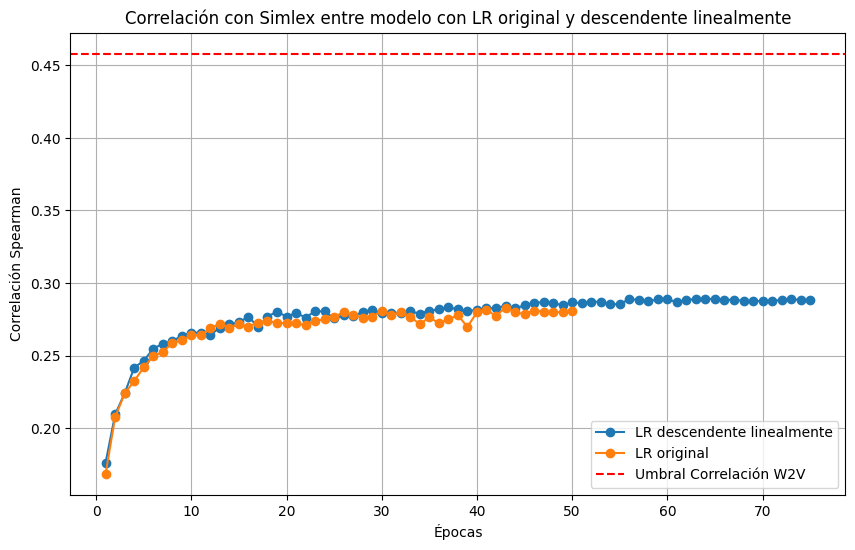
\includegraphics[width=1\textwidth]{imagenes/simlex_corr_lrdescendente.png}
        \caption{}
        \label{fig:simlex_corr_lrdescendente.png}
    \end{subfigure}
    \hfill
    \begin{subfigure}[b]{0.8\textwidth}
        \centering
        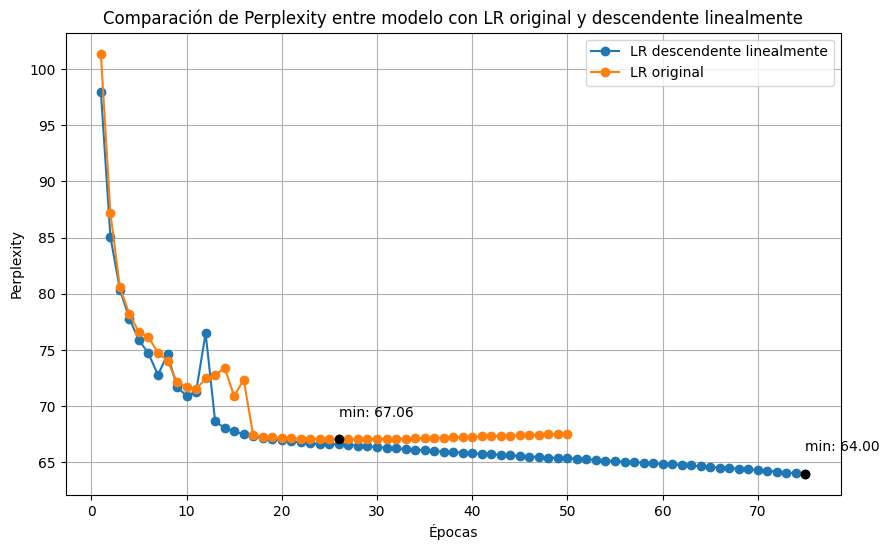
\includegraphics[width=1\textwidth]{imagenes/perp_lr_descendente.png}
        \caption{}
        \label{fig:perp_lr_descendente.png}
    \end{subfigure}
    \caption{Comparación de la correlación con Multi-Simlex a lo largo del entrenamiento 
    entre el modelo de AWD-LSTM presentado en la Figura \ref{fig:10per} y un modelo el cual 
    presenta un \textit{learning rate} el cual desciende linealmente a lo largo de las 
    épocas. En B, se compara la \textit{perplexity} entre ambos modelos.}
    \label{fig:lrdescendente}
\end{figure}

Como se puede observar en la Figura \ref{fig:perp_lr_descendente.png}, mientras que el modelo con el \textit{learning rate} 
original se estanca a partir de una cierta época, el nuevo modelo con el \textit{learning rate} descendiente 
linealmente no solo supera al modelo anterior en \textit{perplexity} dentro de la marca de las $50$ 
épocas, sino que también (al continuar el entrenamiento del modelo) sigue descendiendo 
lentamente gracias a la implementación de un \textit{learning rate} más bajo.

Por otro lado, la correlación con Multi-Simlex del modelo nuevo parece ser idéntica a 
la del modelo anterior, sin presentar mejoras sustanciales. Se puede observar una cierta 
mejora en la correlación en las últimas épocas, pero esto se debe a que el modelo 
nuevo fue entrenado por una cantidad de épocas mayor que el anterior. Incluso 
al compararlo con el umbral obtenido por el modelo de Word2Vec, los resultados 
de los modelos quedan por debajo.

\subsubsection{Síntesis}

Luego de variar varios hiperparámetros e incluso cambiar la forma en la que se elige 
el \textit{learning rate} del modelo a lo largo de las épocas, no se logró igualar los 
niveles de correlación generados por los \textit{embeddings} de Word2Vec. En vista de esto, 
hipotetizamos que probablemente la diferencia entre ambos modelos no sea un 
tema de los hiperparámetros y su entrenamiento en sí, sino más bien que los 
\textit{embeddings} resultantes de la AWD-LSTM son ciertamente distintos a los 
resultantes del modelo Word2Vec, generando resultados disímiles. También 
es una posibilidad que los valores iniciales de la capa de \textit{embeddings} 
de la AWD-LSTM no ayuden al modelo a converger a los resultados esperados.

\subsection{Embeddings preentrenados}

Para poder poner en evidencia esto último, se optó por realizar un experimento 
adicional previo a la elección del modelo base. Uno de los métodos para ayudar 
a un modelo de lenguaje a mejorar su capacidad predictiva durante el entrenamiento 
es aquella de partir con \textit{embeddings} preentrenados por otro modelo y dejar que 
el modelo actual ajuste estos durante el entrenamiento \parencite{Wang2020}. A partir de esto, se decidió entrenar un modelo idéntico al modelo anterior 
durante $10$ épocas, con la salvedad de que esta vez se lo entrenó inicializando 
la capa de \textit{embeddings} de la red neuronal con los \textit{embeddings} provenientes 
del modelo de Word2Vec.

\subsubsection{Resultados}

\begin{figure}[H]
    \centering
    \begin{subfigure}[b]{0.75\textwidth}
        \centering
        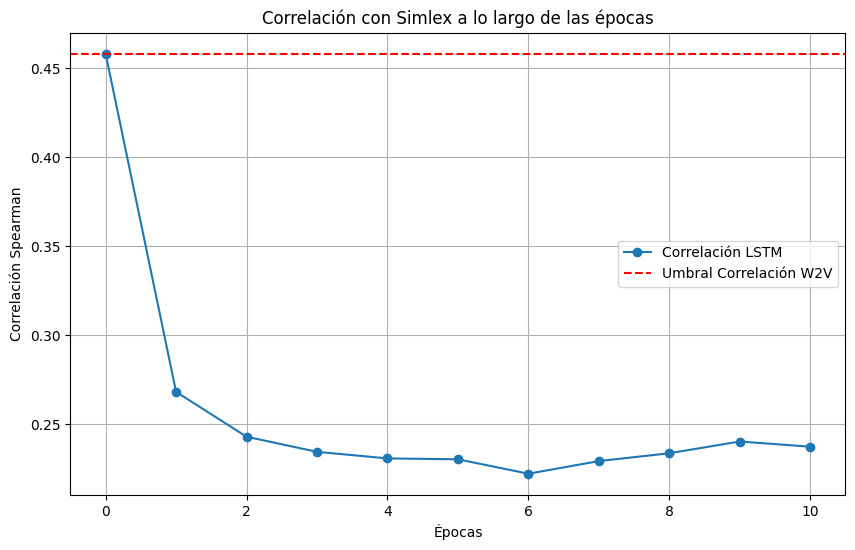
\includegraphics[width=1\textwidth]{imagenes/simlex_corr_preembed.png}
        \caption{}
        \label{fig:simlex_corr_preembed.png}
    \end{subfigure}
    \hfill
    \begin{subfigure}[b]{0.75\textwidth}
        \centering
        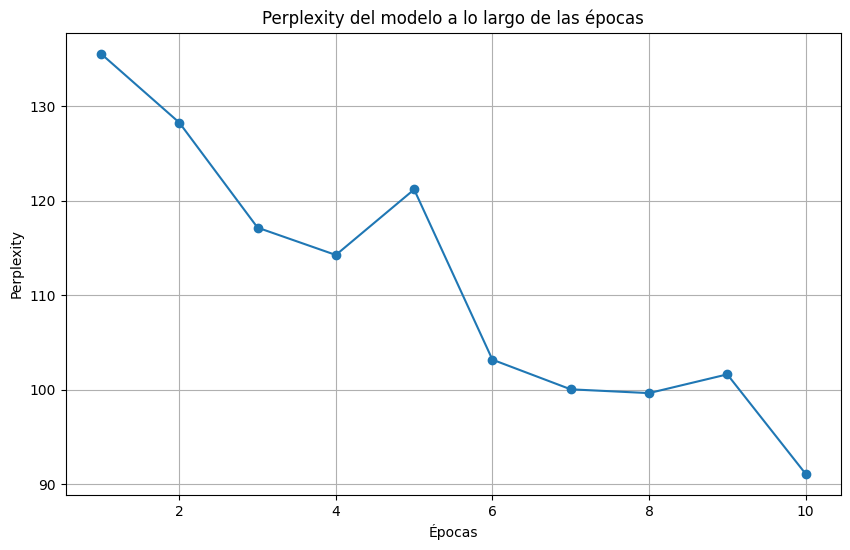
\includegraphics[width=1\textwidth]{imagenes/perp_preembed.png}
        \caption{}
        \label{fig:perp_preembed.png}
    \end{subfigure}
    \caption{En A, se reporta la correlación con Multi-Simlex a lo largo de las épocas 
    del modelo de AWD-LSTM el cual parte de embeddings preentrenados, generados a 
    partir del modelo base de Word2Vec. Nótese que debido a esto, previo al 
    entrenamiento, la correlación con Multi-Simlex es igual que en el modelo 
    de Word2Vec. Por otro lado en B, se reporta la \textit{perplexity} del modelo.}
    \label{fig:preembed}
\end{figure}

Tal y como se puede observar en la Figura \ref{fig:simlex_corr_preembed.png}, la correlación de los 
\textit{embeddings} disminuye drásticamente luego de finalizada la primera época 
de entrenamiento, para luego ir disminuyendo lentamente hasta llegar 
a la época $6$, donde la misma empieza a mejorar levemente. Más aún, también 
se puede observar que la capacidad predictiva del modelo va mejorando 
con el correr de las épocas.

\subsubsection{Síntesis}

A partir de esta información, se concluye que efectivamente los \textit{embeddings} 
extraídos del modelo resultante de la AWD-LSTM se comportan de una manera 
distinta a los de Word2Vec, evidenciado inicialmente en el brusco decrecimiento 
de la correlación con Multi-Simlex luego de terminada la primer época de 
entrenamiento. El modelo no parece estar aprovechando de ninguna manera 
los \textit{embeddings} preentrenados, transformándolos a lo largo del correr de 
las épocas en \textit{embeddings} parecidos a los generados por la AWD-LSTM.

Por otro lado, al observar que la capacidad predictiva del modelo mejora a 
lo largo de las épocas (al contrario que la similitud con Multi-Simlex) nos da 
la pauta de que estos dos resultados no están correlacionados.

\section{Reentrenamiento del modelo base}

\label{sec:reentrenamiento}

Luego de realizadas las experimentaciones pertinentes para lograr hallar un buen 
modelo base sobre el cual reentrenar con información cognitiva, se decidió contar 
con el modelo entrenado a partir de un learning rate linealmente descendente.

A partir de esto, se decidió reentrenar un nuevo modelo utilizándolo como base 
para cada uno de los textos generados a partir de los experimentos con 
movimientos oculares. Estos nuevos modelos fueron reentrenados durante 
$100$ épocas con el 100\% de estos textos, buscando analizar su correspondencia 
con los juicios de similitud humanos utilizados en este trabajo, además 
de compararlos tanto con el modelo base, como con los resultados obtenidos 
en otros modelos, como Word2Vec. En particular, se hicieron comparaciones 
tanto con Multi-Simlex como con SWOW-RP. Para validar el correcto aprendizaje 
de la información cognitiva, también se graficó la correlación de \textit{Spearman} 
entre las predicciones realizadas por el modelo sobre las métricas de 
movimientos oculares para cada época, con el objetivo de ver si los modelos 
lograban aprender a predecir estas métricas a lo largo del entrenamiento.

\subsection{Resultados}

\begin{figure}[H]
    \centering
    \begin{subfigure}[b]{0.8\textwidth}
        \centering
        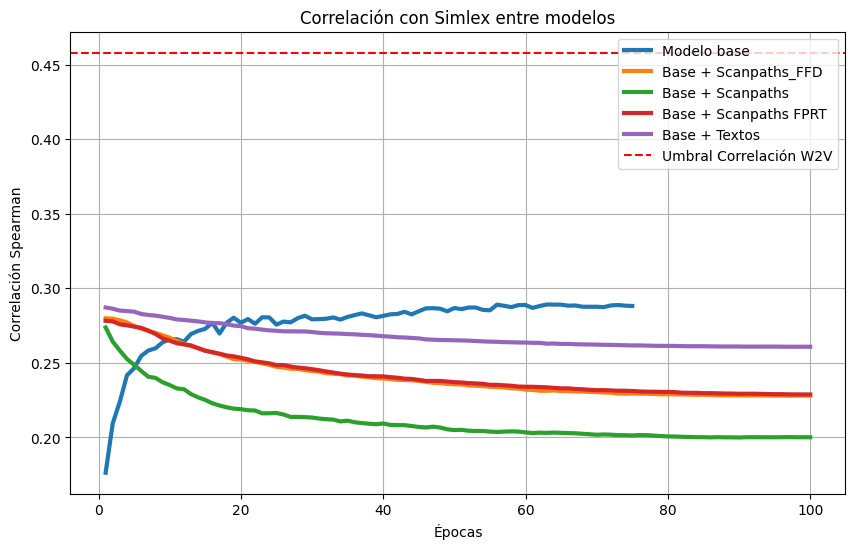
\includegraphics[width=1\textwidth]{imagenes/corr_reentrenamiento.png}
        \caption{}
        \label{fig:corr_reentrenamiento.png}
    \end{subfigure}
    \hfill
    \begin{subfigure}[b]{0.8\textwidth}
        \centering
        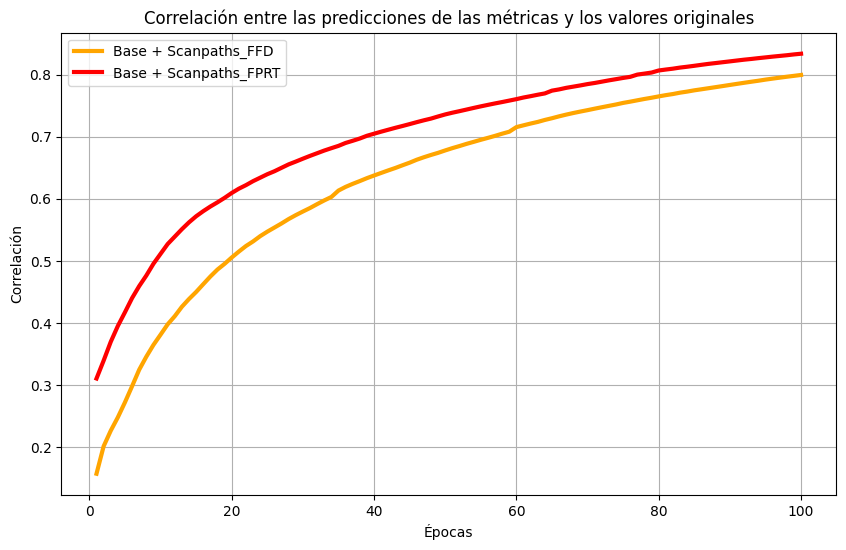
\includegraphics[width=1\textwidth]{imagenes/corr_pred_reentrenamiento.png}
        \caption{}
        \label{fig:corr_pred_reentrenamiento.png}
    \end{subfigure}
    \caption{En A, comparación de la correlación con Multi-Simlex a lo largo de las 
    épocas entre el modelo base elegido y los modelos reentrenados a partir del 
    mismo. En B, para los modelos reentrenados con métricas de movimientos 
    oculares, se reporta la correlación de las predicciones de las métricas 
    generadas por el modelo con los valores originales a lo largo de las épocas.}
    \label{fig:simlex_reentrenamiento}
\end{figure}

A partir de la Figura \ref{fig:corr_reentrenamiento.png} podemos observar que la correlación con Multi-Simlex 
en los modelos reentrenados va disminuyendo paulatinamente a lo largo de 
las épocas, indicando que los \textit{embeddings} generados se van alejando en 
similitud con los datos recabados sobre juicios de similitud humanos. 
Sin embargo, también se puede denotar una diferencia positiva cuando se 
comparan los modelos reentrenados con información cognitiva con el modelo 
reentrenado sin información cognitiva. Por otro lado, en la Figura \ref{fig:corr_pred_reentrenamiento.png}, 
se puede observar que la correlación entre las predicciones de la 
información cognitiva y sus valores originales van aumentando 
considerablemente con el correr de las épocas, dando indicios de que 
el modelo efectivamente está aprendiendo a predecirlas (y, por lo tanto, 
se integran sobre los \textit{embeddings}).

\begin{figure}[H]
    \centering
    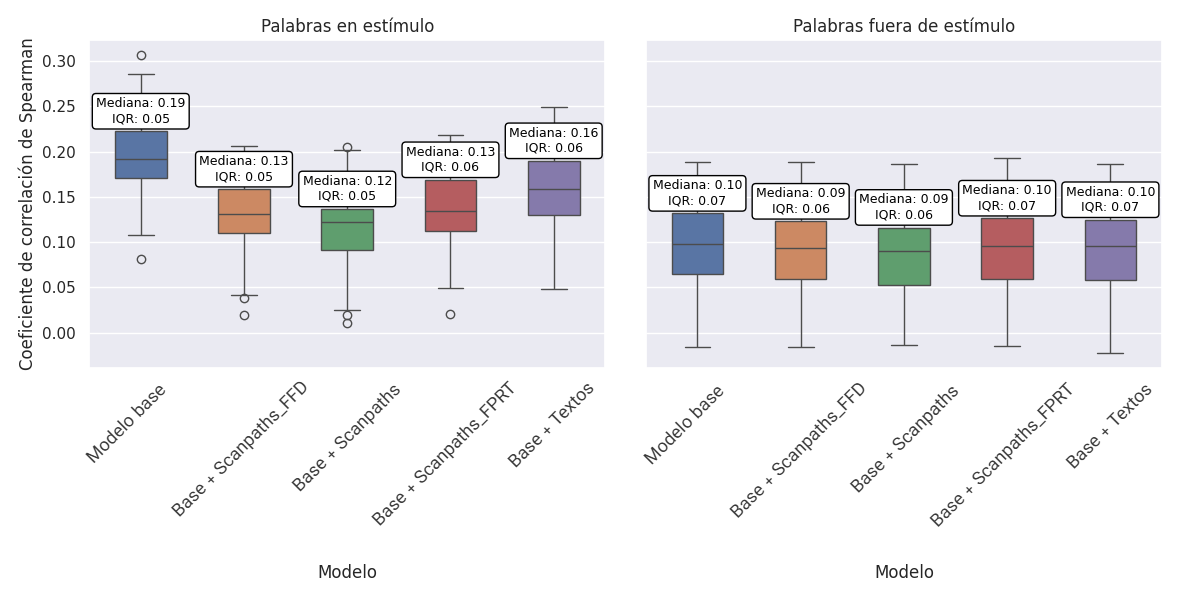
\includegraphics[width=1\textwidth]{imagenes/swow_lstm.png}
    \caption{Comparación de la correlación entre el modelo base y los modelos reentrenados 
    a partir de él con SWOW-RP. Para más rigurosidad estadística, se realiza un 
    muestreo de $1000$ pares de palabras $100$ veces con reposición en vez de 
    comparar todos los pares de palabras una sola vez.}
    \label{fig:swow_lstm}
\end{figure}

Dentro de la correlación con SWOW-RP podemos hallar resultados parecidos 
(Figura \ref{fig:swow_lstm}), donde la correlación es ciertamente menor en los casos en donde 
el modelo es reentrenado, además de contar con una sutil mejora si a ese 
reentrenamiento se lo acompaña con la información relacionada a los experimentos 
sobre movimientos oculares.

Otro resultado que se puede denotar de esto es que si prestamos atención a 
los resultados sobre SWOW-RP por parte de los modelos de Word2Vec (ver \ref{sec:trabajos_previos}), al igual que en el 
caso que con Multi-Simlex, los \textit{embeddings} provenientes del mismo son más 
capaces de captar las similitudes entre pares de palabras puntuadas por los 
humanos que aquellos provenientes de la AWD-LSTM, aunque en el caso de SWOW-RP 
esta diferencia es menos notoria.

\subsection{Síntesis}

A partir de lo observado, se puede llegar a la conclusión que dentro de la 
arquitectura AWD-LSTM los embeddings reentrenados con los \textit{scanpaths} 
empeoran la correlación sobre los juicios de similitud humanos utilizados 
en este trabajo. Sin embargo, se puede observar que la reducción de la similitud 
es menor cuando se incorporan a estos textos de reentrenamiento la información 
cognitiva, dándonos la pauta que quizás el problema no se encuentra en la 
información cognitiva sino en el formato del texto de reentrenamiento. 
Esta hipótesis se vuelve más sólida al observar que, durante el reentrenamiento, 
los \textit{embeddings} efectivamente están aprendiendo a predecir las métricas relacionadas 
con los movimientos oculares, incorporando su información.

Más aún, también se puede cuestionar la utilización de la similitud entre 
pares de palabras como la tarea correcta para evaluar a estos modelos, ya 
que su simpleza puede llegar a evitar que se puedan capturar estas 
mejoras obtenidas con la información cognitiva.





